\documentclass[11pt]{article}
\usepackage{listings}
\usepackage{xcolor}
\definecolor{codegreen}{rgb}{0,0.6,0}
\definecolor{codegray}{rgb}{0.5,0.5,0.5}
\definecolor{codepurple}{rgb}{0.58,0,0.82}
\definecolor{backcolour}{rgb}{0.95,0.95,0.92}
\lstset{
    language=Python,
    keepspaces=true,
    numbers=left,
    backgroundcolor=\color{backcolour},
    commentstyle=\color{codegreen},
    basicstyle=\ttfamily,
    otherkeywords={self,True,False,yield},
    keywordstyle=\ttfamily\color{blue!90!black},
    %basicstyle=\footnotesize,
    keywords=[3]{ttk},
    keywordstyle={[2]\ttfamily\color{orange!80!orange}},
    keywordstyle={[3]\ttfamily\color{red!80!orange}},
    emph={MyClass,__init__},
    emphstyle=\ttfamily\color{red!80!black},
    stringstyle=\color{green!80!black},
    showstringspaces=false
}
\usepackage{enumerate}
\usepackage{fullpage,amsmath,amssymb,graphicx}
\usepackage[colorlinks=true,citecolor=blue,linkcolor=blue]{hyperref} % for href links, and also makes \ref and \eqref clickable in the PDF
\newcommand{\QuasiP}{\mathsf{QuasiP}}
\newcommand{\TIME}{\mathsf{TIME}}
\newcommand{\N}{\mathbb{N}}
\newcommand{\Z}{\mathbb{Z}}
\renewcommand{\P}{\mathsf{P}}
\newcommand{\NP}{\mathsf{NP}}
\newcommand{\poly}{\mathrm{poly}}
\newcommand{\SAT}{\textsc{Sat}}
\newcommand{\sat}{\SAT}
\newcommand{\dnfsat}{\textsc{DNF-\sat}}
\newcommand{\cnfsat}{\textsc{CNF-\sat}}
\newcommand{\pmat}{\textsc{Perfect-Matching}}
\newcommand{\iset}{\textsc{Independent-Set}}
\newcommand{\cpc}{\textsc{Cellphone-Capacity}}
\usepackage{fancyhdr}
\fancypagestyle{firststyle}
{
   \fancyhf{}
   \fancyhead[C]{Copyright \copyright\ \today, David Doty}
}
\title{Homework 3 -- ECS 220, Winter 2020}
\date{}
\newtheorem{theorem}{Theorem}
\newtheorem{lemma}[theorem]{Lemma}
\newtheorem{definition}{Definition}[section]

\begin{document}
\maketitle
\thispagestyle{firststyle}
\vspace{-2.0cm}

\newcommand{\RIS}{\textsc{ReallyIndependentSet}}
\newcommand{\NPC}{\mathsf{NP}\texttt{-complete}}
\newcommand{\tSAT}{\texttt{3-SAT}}

\section{Really independent sets}
    \begin{quote}
    Given a graph $G = (V,E)$, say that a subset $S \subseteq V$ is \emph{really independent} if there are no $u,v \in S$ that are two or fewer steps apart in the graph---that is, if for all $u,v \in S$, the length of the shortest path
    between $u$ and $v$ is at least 3.
    The problem \textsc{ReallyIndependentSet} takes a graph $G$ and an integer $k$ as input, and asks if $G$ has a really independent set of size $k$ or more.
    Prove that \textsc{ReallyIndependentSet} is $\NP$-complete.
    \end{quote}

We would be proofing $\RIS \in \NPC$ by reducing $\tSAT$ to it. 

\begin{theorem}
    $\RIS \in \NP $
\end{theorem}

\begin{proof}
    A brute force enumeration over all possible combination over $k$ nodes would take $O(C^k_{|V|})$, for each possibility, the time to verify it would be $O(1)$ if we pre-compute a distance map between all pairs of nodes.
    Therefore, we can say $\RIS \in \NP$
    
    P.S. It's trivial that if a $\RIS$ of size $k+1$ exists, a $\RIS$ of size $k$ must exist, thus we don't enumerate combinations with size larger than $k$.
\end{proof}

\begin{definition}{Reduction}
    Suppose we are given a $\tSAT$ problem with $k$ clauses.

    For each clause we construct a 3-clique. With each node labelled itself or it's negation depends on the clause.
    Now we have $k$ 3-cliques, find all negation pairs(i.e. nodes labelled with $a$ and $-a$), add a dummy node $D$ and connect $D$ with both nodes.

    Finally, connect all dummy nodes $D$.
\end{definition}

\textbf{Example} The follow image shows how a $\tSAT$ $F = (a \vee b \vee c) \wedge (-c \vee d \vee e) \wedge (-a\vee -c \vee d)$ is converted into a graph.

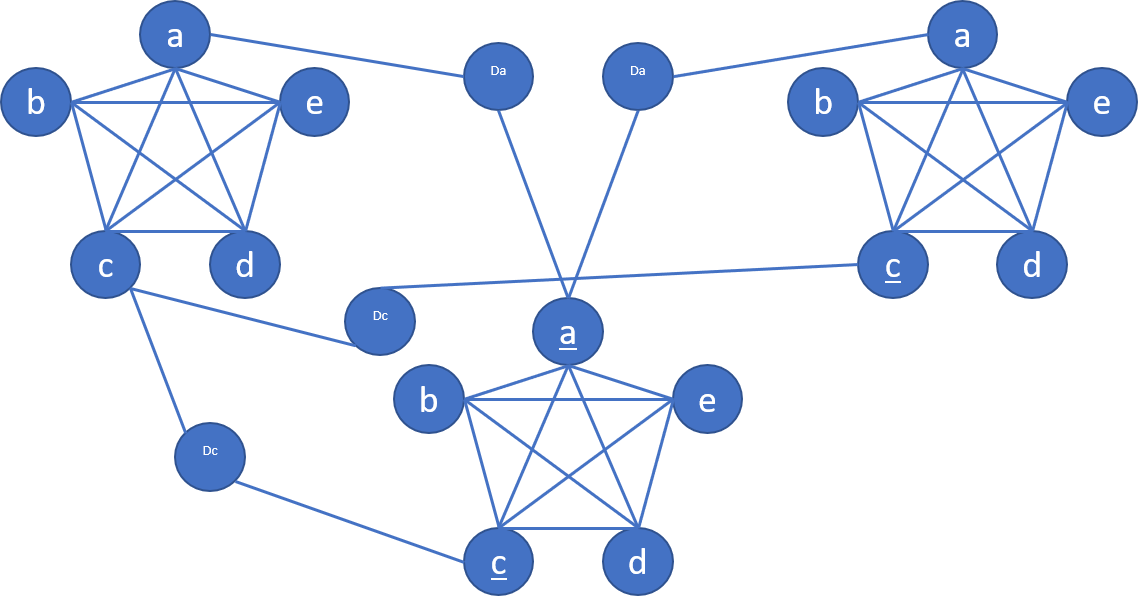
\includegraphics[width = \textwidth]{Ex1.png}

The intuition behind the reduction is that any variable cannot have itself coexist with its negation, so all pairs of non-negation and negation variable has a distance of 2. 
Meanwhile we have to set the distance to 2 instead of 1 or we might have different variables having a distance less than 3.

\begin{theorem}
    Reduction is in $\P$
\end{theorem}

\begin{proof}
    For $k$ 3-cliques, the total time required is linear to $k$, therefore $O(k)$.

    For each variable, suppose out of $k$ clauses, there are only $s$ of them and $t$ of them are negated, then we would add $t(s-t) \leq O(k^2)$ nodes since $s \leq 3k$, $t \leq 3k$. 
    There are at most $3k$ different variables, so the maximum complexity is $O(k^3)$.

    Therefore the total time for this reduction would be $O(k^3)$.
\end{proof}

\begin{lemma}
    If such reduced graph has $\RIS$ of size $k$, there will be no dummy node $D$ in $\RIS$
\end{lemma}

\begin{proof}
    \textit{Note}: This lemma comes handy when proving $\Leftarrow$ direction in the next proof. 

    Suppose there is dummy node $D$. 
    Then we have the following consequences:
    \begin{enumerate}
        \item The two 3-clique connected by $D$ will have a distance to $D$ less equal than 2. 
        \item All other dummy nodes cannot be picked.
        \item Any other 3-clique have a distance to $D$ with a distance of 2 or 3, no more.
    \end{enumerate}
    
    Then the $\RIS$ of this graph is at most $k-1$ since there are only $k$ 3-cliques.

    Therefore, dummy node $D$ cannot be selected into $\RIS$ is there is one.
\end{proof}

\begin{theorem}
    $\tSAT$ is satisfiable iff the reduced graph has $\RIS$.
\end{theorem}

\begin{proof}
    $\Rightarrow$
    
    Suppose we have a set of solutions to $\tSAT$, then for each clause there must be at least one node evaluates to true.
    In each clique, we randomly select ONE such true node. The set of all nodes selected from each 3-clique would be $\RIS$.

    It is easy to see that all pairs of selected nodes must have a distance larger than 2: The connection between two clique take distance of 2 and the directly connected nodes cannot be picked at the same time as they are the negation of each other.

    Example: Think of the distance between $c$ and $d$ in the example, both distance is 3(except for the $d$ in the same clique.)

    $\Leftarrow$

    Since dummy node $D$ cannot be selected as we have proved in the lemma above, in each 3-clique the distance between all nodes is 1. 
    Then the only possible way to form a $\RIS$ is by selecting one node in each clique.
    We claim that the selected nodes, when setting corresponding variable to true, $\tSAT$ will be solved.

    First let's proof that the selected nodes are not conflicting, i.e. $a$ and $-a$ cannot be selected at the same time.
    Per the definition of $\RIS$, this is trivial as any negation nodes have distance of 2.

    Then let's proof that the selected nodes do solve $\tSAT$.
    In each 3-clique one node is selected to be true, and therefore corresponding clause is true. 
    Since all 3-clique got one node selected, all clauses are true.
\end{proof}

Therefore, we have proved  that $\tSAT \le_P \RIS$, and thus, $$\RIS \in \NPC$$

\end{document}
